\documentclass{standalone}

\usepackage{amsmath}
\usepackage{hyperref}
\usepackage{tikz}
\usepackage{graphicx}
\usepackage{relsize}
\usepackage[T1]{fontenc}
% \usepackage{tgheros}
% \renewcommand{\rmdefault}{qhv}
% \usepackage[symbolgreek]{mathastext}

\usetikzlibrary{decorations.pathreplacing,
  arrows,
  calc,
  decorations.pathmorphing,
  decorations.pathreplacing,
  decorations.markings,
  fadings,
  positioning,
  shapes,
  arrows.meta
}
\tikzstyle{snakearrow} = [decorate, decoration={pre length=0.1cm,
  post length=0.1cm, snake, amplitude=.4mm,
  segment length=4mm},thick, ->]
\tikzstyle{tightsnakearrow} = [decorate, decoration={pre length=0.1cm,
  post length=0.1cm, snake, amplitude=.2mm,
  segment length=2mm},thick, ->]
\usepgfmodule{oo}

\pgfdeclareradialshading{glow2}{\pgfpoint{0cm}{0cm}}{
  color(0mm)=(white);
  color(2mm)=(white);
  color(8mm)=(black);
  color(10mm)=(black)
}
\pgfdeclareradialshading{glow}{\pgfpoint{0cm}{0cm}}{
  color(0mm)=(white);
  color(5mm)=(white);
  color(9mm)=(black);
  color(10mm)=(black)
}

\begin{tikzfadingfrompicture}[name=glow fading]
  \shade [shading=glow] (0,0) circle (1);
\end{tikzfadingfrompicture}

\begin{tikzfadingfrompicture}[name=glow2 fading]
  \shade [shading=glow2] (0,0) circle (1);
\end{tikzfadingfrompicture}

\definecolor{atomorange}{rgb}{1.0,0.483,0.0}
\definecolor{pyplotc0}{rgb}{0.122,0.467,0.706}
\definecolor{pyplotc1}{rgb}{1.000,0.498,0.055}
\definecolor{pyplotc2}{rgb}{0.173,0.627,0.173}
\definecolor{pyplotc3}{rgb}{0.839,0.153,0.157}
\definecolor{pyplotc4}{rgb}{0.580,0.404,0.741}
\definecolor{pyplotc5}{rgb}{0.549,0.337,0.294}
\definecolor{pyplotc6}{rgb}{0.890,0.467,0.761}
\definecolor{pyplotc7}{rgb}{0.498,0.498,0.498}
\definecolor{pyplotc8}{rgb}{0.737,0.741,0.133}
\definecolor{pyplotc9}{rgb}{0.090,0.745,0.812}

\pgfdeclarelayer{tweezer}
\pgfsetlayers{tweezer,main}
\pgfooclass{tweezer}{
  \method tweezer() {
  }
  \method drawTweezer(#1,#2,#3) {
    \shade[shading=radial,path fading=glow fading,shift={(#1,#2)},rotate=90,yscale=1,
    fill opacity=0.9,inner color=#3]
    plot[draw,samples=200,domain=-4.5:4.5] function {sqrt(0.02 + (x)**2 / 10)}
    -- plot[draw,samples=200,domain=4.5:-4.5] function {-sqrt(0.02 + (x)**2 / 10)};
  }
  \method drawRaman(#1,#2) {
    \pgfoothis.drawTweezer(#1,#2,pyplotc4);
  }
  \method drawAtom(#1,#2,#3,#4) {
    \fill [#4,path fading=glow2 fading] (#1,#2) circle (#3);
  }
  \method drawDownAtom(#1,#2,#3) {
    \pgfoothis.drawAtom(#1,#2,#3,pyplotc0);
  }
  \method drawUpAtom(#1,#2,#3) {
    \pgfoothis.drawAtom(#1,#2,#3,pyplotc1);
  }
  \method drawElement(#1,#2,#3,#4,#5,#6) {
    \node[fill=#4,fill opacity={#5 * #6},text opacity=#6,rounded corners=1,inner sep=5] at (#1, #2) {#3};
  }
}
\pgfoonew \mytweezer=new tweezer()

\ifpdf
  % Ensure reproducible output
  \pdfinfoomitdate=1
  \pdfsuppressptexinfo=-1
  \pdftrailerid{}
  \hypersetup{
    pdfcreator={},
    pdfproducer={}
  }
\fi

\begin{document}
\begin{tikzpicture}
  \def\DX{1.55}
  \def\DY{-0.95}
  \mytweezer.drawElement(\DX*0, \DY*0, {${\mathlarger{\rho}}_{\downarrow\!E,\downarrow\!E}$}, pyplotc0, 0.5, 1);
  \mytweezer.drawElement(\DX, \DY*0, {${\mathlarger{\rho}}_{\downarrow\!E,\uparrow\!E}$}, white, 0, 0.2);
  \mytweezer.drawElement(\DX*2, \DY*0, {${\mathlarger{\rho}}_{\downarrow\!E,\downarrow\!L}$}, white, 0, 0.2);
  \mytweezer.drawElement(\DX*3, \DY*0, {${\mathlarger{\rho}}_{\downarrow\!E,\uparrow\!L}$}, pyplotc3, 0.5, 1);

  \mytweezer.drawElement(\DX*0, \DY*1, {${\mathlarger{\rho}}_{\uparrow\!E,\downarrow\!E}$}, white, 0, 0.2);
  \mytweezer.drawElement(\DX, \DY*1, {${\mathlarger{\rho}}_{\uparrow\!E,\uparrow\!E}$}, pyplotc2, 0.5, 1);
  \mytweezer.drawElement(\DX*2, \DY*1, {${\mathlarger{\rho}}_{\uparrow\!E,\downarrow\!L}$}, pyplotc1, 0.5, 1);
  \mytweezer.drawElement(\DX*3, \DY*1, {${\mathlarger{\rho}}_{\uparrow\!E,\uparrow\!L}$}, white, 0, 0.2);

  \mytweezer.drawElement(\DX*0, \DY*2, {${\mathlarger{\rho}}_{\downarrow\!L,\downarrow\!E}$}, white, 0, 0.2);
  \mytweezer.drawElement(\DX, \DY*2, {${\mathlarger{\rho}}_{\downarrow\!L,\uparrow\!E}$}, pyplotc1, 0.5, 1);
  \mytweezer.drawElement(\DX*2, \DY*2, {${\mathlarger{\rho}}_{\downarrow\!L,\downarrow\!L}$}, pyplotc2, 0.5, 1);
  \mytweezer.drawElement(\DX*3, \DY*2, {${\mathlarger{\rho}}_{\downarrow\!L,\uparrow\!L}$}, white, 0, 0.2);


  \mytweezer.drawElement(\DX*0, \DY*3, {${\mathlarger{\rho}}_{\uparrow\!L,\downarrow\!E}$}, pyplotc3, 0.5, 1);
  \mytweezer.drawElement(\DX, \DY*3, {${\mathlarger{\rho}}_{\uparrow\!L,\uparrow\!E}$}, white, 0, 0.2);
  \mytweezer.drawElement(\DX*2, \DY*3, {${\mathlarger{\rho}}_{\uparrow\!L,\downarrow\!L}$}, white, 0, 0.2);
  \mytweezer.drawElement(\DX*3, \DY*3, {${\mathlarger{\rho}}_{\uparrow\!L,\uparrow\!L}$}, pyplotc0, 0.5, 1);
\end{tikzpicture}
\end{document}
